\section{球面化}
荷重が適切に測定できるようにラティス構造とセンサ部が接触する面の球面化を提案する.従来ではラティス構造とセンサ部は平面で接触しているため力の分散が考えられる測定困難であるとされたが接触面を球面化することにより荷重が集中し測定が可能になると考えられる.そこで球面化柔軟指(変更予定)	と名付けた指を\refig{semi_finger}に示す.半球形の把持部の中に先に述べた指と同じパラメータのラティス構造設計した.


\begin{figure}[h]
\centering
\subfloat[横]{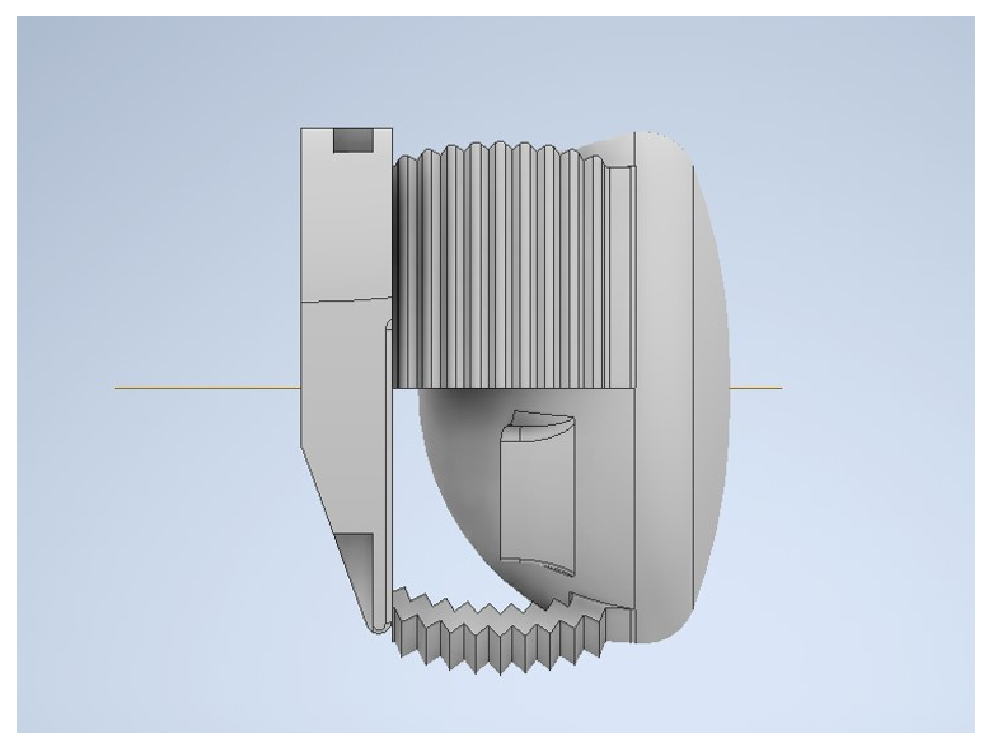
\includegraphics[scale=0.4]{../fig/eps/semi_finger.eps}}
\hspace{5mm}
\subfloat[正面]{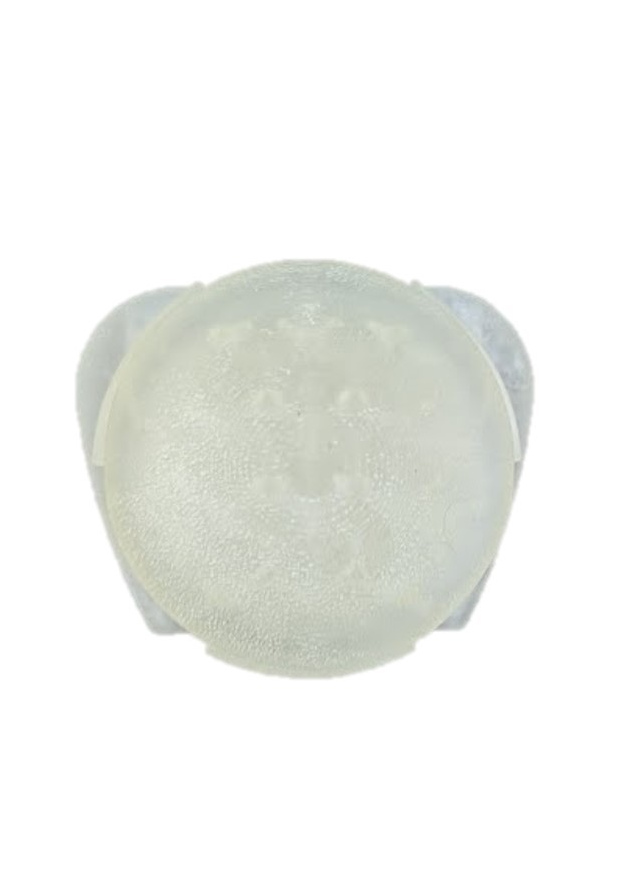
\includegraphics[scale=0.4]{../fig/eps/semi_finger_b.eps}}
\caption{球面化柔軟指}
\label{fig::semi_finger}
\end{figure}

\subsection{荷重実験}
球面化柔軟指に力覚センサを取り付け荷重を測定する.

\subsection{比較実験}


